\section{Uždaviniai}

\begin{figure}
  \centering
	\subfloat[Be užlaikymo]{
		\label{fig:disappear}
		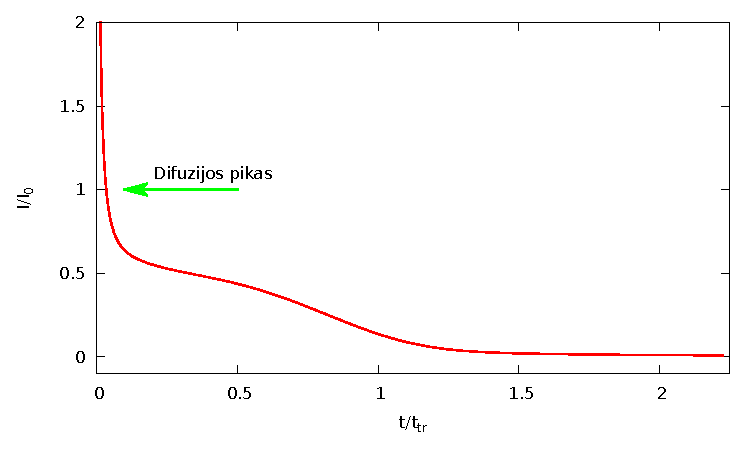
\includegraphics[width=0.5\textwidth]{./media/pdf/disappear.pdf}
		}
	\subfloat[Su užlaikymu]{
		\label{fig:exist}
		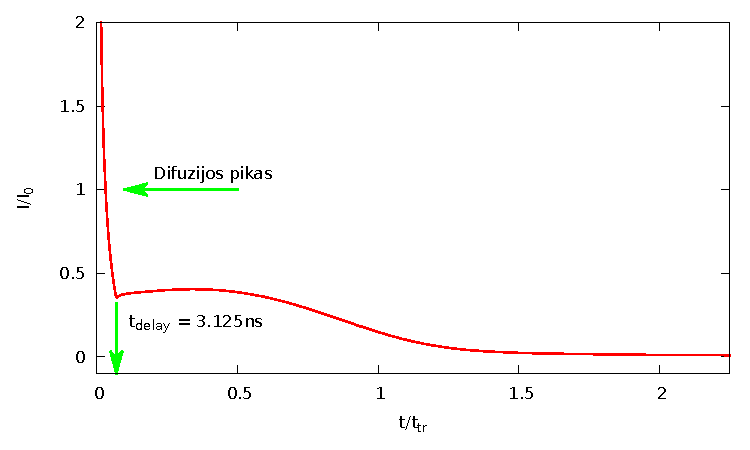
\includegraphics[width=0.5\textwidth]{./media/pdf/exist.pdf}
		}
  \caption{Difuzijos pikas matomas photo-CELIV srovės kinetikoje}
  \label{fig:celiv_example}
\end{figure}

Praeitame darbe \cite{vytis:kursinis} nustatyta, jog esant paviršinei šviesos sugerčiai $(\alpha d > 1)$ sudaromi pakankami krūvininkų pasiskirstymo gradientai, kad modeliuojamose photo-CELIV kinetikose matytųsi difuzinė srovės komponentė (žr. \ref{fig:celiv_example} pav.). Taip pat pastebėta, jog difuzijos komponentė keičia kinetikos maksimumo padėtį ir vertę.

Kai kurie fizikiniai dydžiai gali būti skaičiuojami pagal kinetikos maksimumo vertę ir padėtį, taigi dėl difuzijos komponentės gali kisti šių matavimų rezultatai: rekombinacijos koeficiento ir judrio.

\subsection{Rekombincijos matavimai}

Rekombinacijos koeficientas gali būti nustatytas pagal kinetikos maksimumo vertės sotinimasį nuo generuojamų krūvininkų kiekio \cite{juška:155202}. Difuzijos įtakos įvertinimui suskaičiuosime photo-CELIV kinetikas įskaitant difuziją ir be jos. Iš šių kinetikų suskaičiuosime rekombinacijos koeficientą ir palyginsime su tikruoju, kuris naudotas skaičiavimuose.

\paragraph{Skaičiavimų ribojimai}
Įtraukus difuziją pastebėta, jog esant paviršinei sugerčiai pradinis difuzinės srovės pikas "praryja" srovės maksimumą (žr. \ref{fig:disappear} pav.).
Norėdami to išvengti visus soties vertės skaičiavimus atlikome su kiek įmanoma mažu uždelsimo laiku $t_{delay} = 3.125ns$, tam kad atskirti pradinį difuzijos piką ir CELIV kinetiką (žr. \ref{fig:exist} pav.). Toks sprendimas nepakeičia suskaičiuotų rezultatų svarbos, nes labai dažnai realaus eksperimento metu egzistuoja laiko tarpas tarp šviesos impulso ir įtampos impulso.

\subsection{Judrio matavimai}
Photo-CELIV maksimumo padėtis leidžia nustatyti krūvininkų judrį pagal sąryšį:
\begin{equation}
\label{eq:judris}
\mu = \frac{2d^2}{At_{max}^2}
\end{equation}

Pasinaudodami suskaičiuotomis srovės kinetikomis, pagal \eqref{eq:judris} formulę suskaičiuosime krūvininkų judrį ir palyginsime su tikruoju parametru, kuris naudotas skaičiavimuose. Šiuose skaičiavimuose neįtrauksime pataisos koeficiento K \cite{juška:155202}, nes tirsime judrio skaičiavimo validumą esant užlaikymo laikui $t_{delay}$ ir difuzijai.

